\documentclass[11pt,a4paper]{article}

% ============================================================
% Packages
% ============================================================
\usepackage[utf8]{inputenc}
\usepackage[T1]{fontenc}
\usepackage{amsmath,amssymb,amsfonts}
\usepackage{graphicx}
\usepackage{booktabs}
\usepackage{hyperref}
\usepackage{xcolor}
\usepackage{algorithm}
\usepackage{algpseudocode}
\usepackage{subcaption}
\usepackage{multirow}
\usepackage[margin=1in]{geometry}
\usepackage{natbib}
\usepackage{enumitem}

\hypersetup{
    colorlinks=true,
    linkcolor=blue!70!black,
    citecolor=green!50!black,
    urlcolor=blue!60!black
}

% Custom commands
\newcommand{\astria}{\textsc{Astria}}
\newcommand{\concept}{\mathcal{C}}
\newcommand{\encoder}{f_\theta}
\newcommand{\policy}{\pi_\phi}
\newcommand{\KL}{\mathrm{KL}}

\title{
\textbf{\astria: Unsupervised Concept Bottleneck Models\\for Interpretable Reinforcement Learning}
}

\author{
Thomas Pravetz\\
\texttt{github.com/tompravetz/astria}
}

\date{February 2026}

\begin{document}
\maketitle

% ============================================================
% Abstract
% ============================================================
\begin{abstract}
We present \astria{} (\textbf{A}utonomous \textbf{St}rategy \textbf{R}easoning via \textbf{I}nterpretable \textbf{A}gents), a framework for building interpretable reinforcement learning agents through unsupervised concept bottleneck models. While prior work on concept bottleneck models in RL relies on supervised, domain-specific concept labels, \astria{} discovers concepts automatically through K-means clustering of learned encoder features---requiring \emph{zero human supervision}. We introduce a three-stage pipeline: (1) train a standard RL encoder, (2) discover discrete concepts via unsupervised clustering, and (3) train a bottleneck policy that receives \emph{only} a concept ID as input. We additionally explore an end-to-end variant using Vector Quantization (VQ-VAE). Evaluated on Go~7$\times$7 and CartPole with both PPO and DQN, our bottleneck agents achieve 96--100\% win rates while maintaining full interpretability. Causal intervention experiments demonstrate that concepts are causally meaningful (75.6\% action change rate, $p < 10^{-151}$), ablation studies identify two strategically critical concepts, and an information bottleneck sweep reveals that as few as 16 concepts (4 bits) achieve 97\% win rate. Cross-domain experiments on CartPole confirm task-agnosticism. Our results show that unsupervised concept discovery can produce causally grounded, interpretable representations in RL without requiring domain expertise to define concept labels.
\end{abstract}

\textbf{Keywords:} Interpretable Reinforcement Learning, Concept Bottleneck Models, Unsupervised Concept Discovery, Vector Quantization, Causal Interpretability

% ============================================================
% 1. Introduction
% ============================================================
\section{Introduction}

Reinforcement learning (RL) agents can achieve superhuman performance in complex domains~\citep{silver2017mastering, berner2019dota}, yet their decision-making processes remain largely opaque. This opacity limits deployment in safety-critical domains and hinders scientific understanding of learned strategies. The fundamental challenge is clear: \emph{how can we build RL agents whose reasoning is transparent without sacrificing performance?}

Concept Bottleneck Models (CBMs)~\citep{koh2020concept} address this in supervised learning by forcing predictions through an intermediate layer of human-interpretable concepts. Recent work has extended this idea to RL: Delfosse et al.~\citep{delfosse2024interpretable} introduced SCoBots, which use \emph{supervised} object-centric concepts (e.g., ball position, paddle angle) to build interpretable Atari agents. However, their approach requires domain experts to predefine concept labels for each environment---a significant limitation that restricts applicability to domains where such labels exist.

We propose \astria{}, a framework that eliminates this supervision requirement entirely. Our key insight is that a trained RL encoder already learns features that capture strategically relevant information about game states. By applying unsupervised clustering (K-means) to these learned features, we can discover discrete concepts \emph{without any human labels}. The resulting concept bottleneck forces the policy to act based solely on a single discrete concept ID, creating a fully interpretable decision pipeline:
\[
\text{Observation} \xrightarrow{\text{Frozen Encoder}} \text{128D Features} \xrightarrow{\text{K-means}} \text{Concept ID} \xrightarrow{\text{Bottleneck Policy}} \text{Action}
\]

Our contributions are:
\begin{enumerate}[leftmargin=*]
    \item \textbf{Unsupervised concept discovery for RL}: We show that K-means clustering of encoder features produces causally meaningful concepts without human supervision, unlike prior work requiring predefined concept labels.
    \item \textbf{Three-stage bottleneck pipeline}: A modular framework that can be applied to any RL encoder, separating feature learning from concept discovery from policy training.
    \item \textbf{End-to-end VQ-VAE variant}: A differentiable alternative using Vector Quantization with straight-through estimation, enabling joint optimization of encoder and concept space.
    \item \textbf{Comprehensive causal evaluation}: Intervention, ablation, and dynamics experiments that validate concept causality across two domains (Go~7$\times$7 and CartPole) and two algorithms (PPO and DQN).
\end{enumerate}

% ============================================================
% 2. Related Work
% ============================================================
\section{Related Work}

\paragraph{Concept Bottleneck Models.}
Koh et al.~\citep{koh2020concept} introduced CBMs for supervised learning, where models predict human-defined concepts as an intermediate step before making final predictions. This enables concept-level interventions at test time. Extensions include stochastic CBMs~\citep{kim2023stochastic} that handle concept uncertainty, energy-based CBMs~\citep{xu2024energy} that improve expressiveness, and probabilistic CBMs~\citep{kim2023probabilistic} with better calibration. All of these require supervised concept labels during training.

\paragraph{Interpretable Reinforcement Learning.}
Delfosse et al.~\citep{delfosse2024interpretable} extended CBMs to RL with SCoBots, using object-centric concepts (positions, velocities, relations between game objects) to build interpretable Atari agents. Their approach achieves strong performance but requires domain-specific concept engineering---each new environment needs hand-designed concept extractors. In contrast, \astria{} discovers concepts automatically from any trained encoder.

\paragraph{Discrete Representations in RL.}
Vector Quantized representations have gained traction in RL for learning discrete state abstractions. VQ-VLA~\citep{zhu2024vqvla} uses VQ for robotic manipulation, while Hafner et al.~\citep{hafner2020dreamer} employ categorical latent variables in world models. SINDy-RL~\citep{zolman2025sindyrl} learns symbolic representations for interpretable dynamics. Our VQ-VAE variant connects to this line of work, but with the specific goal of creating an interpretable concept bottleneck rather than general state compression.

\paragraph{Causal Interpretability.}
Causal approaches to understanding neural networks~\citep{geiger2021causal} test whether internal representations have causal effects on behavior, rather than merely correlating with outputs. Our intervention experiments directly test causal influence: overriding concept assignments and measuring behavioral change. This goes beyond saliency maps or attention visualization by providing \emph{causal}, not correlational, evidence of concept importance.

% ============================================================
% 3. Method
% ============================================================
\section{Method}

\subsection{Overview}

\astria{} operates in three stages, each producing a reusable artifact:

\begin{enumerate}[leftmargin=*]
    \item \textbf{Stage 1 --- Baseline Training}: Train a standard RL agent (PPO or DQN) with a CNN/MLP encoder $\encoder$, producing a frozen encoder that maps observations to 128-dimensional feature vectors.
    \item \textbf{Stage 2 --- Concept Discovery}: Collect features $\{z_i = \encoder(o_i)\}_{i=1}^N$ from gameplay episodes, then fit K-means with $K=64$ clusters to discover concept centroids $\{\mu_k\}_{k=1}^K$.
    \item \textbf{Stage 3 --- Bottleneck Training}: Train a new policy $\policy$ that receives \emph{only} a concept ID $c = \arg\min_k \|z - \mu_k\|_2$ as input, implemented as an embedding lookup followed by an MLP.
\end{enumerate}

\subsection{Stage 1: Baseline Encoder Training}

We train standard RL baselines using Stable Baselines 3~\citep{raffin2021stable} for PPO and a custom implementation for DQN. For Go~7$\times$7, we use a CNN encoder with the following architecture:

\begin{align}
    z &= \encoder(o) = \text{FC}_{128}(\text{ReLU}(\text{Flatten}(\text{Conv}_{64}(\text{Conv}_{32}(o))))) \label{eq:encoder}
\end{align}

where $o \in \mathbb{R}^{7 \times 7 \times 3}$ encodes black stones, white stones, and empty positions. The encoder output $z \in \mathbb{R}^{128}$ is shared between the policy and value heads.

\paragraph{Augmented Training.}
Go boards have 8-fold symmetry under the dihedral group $D_4$ (4 rotations $\times$ 2 reflections). We apply random symmetry transformations during training to encourage rotation-invariant features, with corresponding action remapping to maintain consistency:
\begin{equation}
    o' = T_g(o), \quad a' = g(a), \quad g \sim \text{Uniform}(D_4)
\end{equation}

\subsection{Stage 2: Concept Discovery via K-Means}

After freezing the encoder, we collect feature vectors from 500 episodes of random play and 500 episodes of policy play, yielding approximately 30,000--60,000 feature vectors. We then fit MiniBatch K-means with $K=64$ clusters:

\begin{equation}
    c(o) = \arg\min_{k \in \{0, \ldots, K-1\}} \| \encoder(o) - \mu_k \|_2
\end{equation}

This discretization creates the information bottleneck: all downstream decisions are based solely on which of 64 clusters the current state falls into. The choice of $K=64$ balances expressiveness (enough concepts to capture diverse strategies) with interpretability (few enough to analyze individually).

\subsection{Stage 3: Bottleneck Policy}

The bottleneck policy receives a single integer $c \in \{0, \ldots, 63\}$ and outputs action probabilities:

\begin{equation}
    \policy(a \mid c) = \text{Softmax}(\text{MLP}(\text{Embed}(c)))
\end{equation}

where $\text{Embed}: \{0, \ldots, 63\} \to \mathbb{R}^{64}$ is a learned embedding and the MLP has one hidden layer of 128 units with ReLU activation. This architecture has only $\sim$15,000 parameters, compared to $\sim$100,000 for the full baseline.

We train the bottleneck policy using generational training: 100 generations of 20,000 timesteps each, collecting concept-action-outcome triplets into a strategy memory for post-hoc analysis.

\subsection{End-to-End Variant: VQ-VAE Concepts}

As an alternative to the three-stage pipeline, we explore end-to-end concept learning using Vector Quantization (VQ)~\citep{van2017neural}. The VQ layer replaces K-means with a differentiable discretization:

\begin{equation}
    z_q = e_{k^*}, \quad k^* = \arg\min_k \| z_e - e_k \|_2
\end{equation}

where $z_e = \encoder(o)$ is the encoder output and $\{e_k\}_{k=1}^K$ is the learnable codebook. Gradients flow through via the straight-through estimator~\citep{bengio2013estimating}, and the codebook is updated with exponential moving averages (EMA):

\begin{equation}
    \mathcal{L}_{\text{VQ}} = \| \text{sg}[z_e] - z_q \|_2^2 + \beta \| z_e - \text{sg}[z_q] \|_2^2
\end{equation}

where $\text{sg}[\cdot]$ denotes stop-gradient and $\beta = 0.25$ is the commitment cost.

% ============================================================
% 4. Experimental Setup
% ============================================================
\section{Experimental Setup}

\subsection{Environments}

\paragraph{Go 7$\times$7.}
We use the PettingZoo~\citep{terry2021pettingzoo} implementation of Go, wrapped as a single-agent Gymnasium environment. The observation space is $\mathbb{R}^{7 \times 7 \times 3}$ (binary planes for black/white/empty), and the action space has 50 discrete actions (49 board positions + pass). The agent plays black against a mix of random opponents and self-play opponents (past versions of the bottleneck agent), with self-play introduced after generation 10 at a 50\% ratio.

\paragraph{CartPole-v1.}
The classic control task with continuous 4D observations and 2 discrete actions. We use an MLP encoder ($4 \to 64 \to 128$) and $K=32$ concepts to test cross-domain generalization.

\subsection{Algorithms}

We compare two RL algorithms across both environments:
\begin{itemize}[leftmargin=*]
    \item \textbf{PPO}~\citep{schulman2017proximal}: On-policy actor-critic via Stable Baselines 3 with MaskablePPO for legal move enforcement in Go.
    \item \textbf{DQN}~\citep{mnih2015human}: Off-policy Q-learning with a custom implementation supporting action masking, reward shaping (small bonuses for captures), and $\epsilon$-greedy exploration.
\end{itemize}

\subsection{Evaluation Metrics}

We design five experiments to validate concept quality from different angles:

\begin{enumerate}[leftmargin=*]
    \item \textbf{Causal Intervention} (Section~\ref{sec:intervention}): Override concept assignments and measure action change rate.
    \item \textbf{Concept Ablation} (Section~\ref{sec:ablation}): Disable individual concepts and measure win rate impact.
    \item \textbf{Concept Stability} (Section~\ref{sec:stability}): Test invariance under board symmetries.
    \item \textbf{Concept Dynamics} (Section~\ref{sec:dynamics}): Train a next-concept predictor to test temporal structure.
    \item \textbf{Cross-Domain Transfer} (Section~\ref{sec:cartpole}): Replicate experiments on CartPole.
\end{enumerate}

% ============================================================
% 5. Results
% ============================================================
\section{Results}

\subsection{Bottleneck Agent Performance}

\begin{table}[t]
\centering
\caption{Performance comparison of concept bottleneck agents. Win rates measured over 50 games against a random opponent. ``Best'' indicates peak win rate during training; ``Final'' is the last generation. PPO trained with self-play (50\% of generations use past agent versions as opponents).}
\label{tab:performance}
\begin{tabular}{lccc}
\toprule
\textbf{Metric} & \textbf{PPO Bottleneck} & \textbf{DQN Bottleneck} & \textbf{VQ End-to-End} \\
\midrule
Win Rate (Best)       & \textbf{100\%} & 96\%  & 92\% \\
Win Rate (Final)      & \textbf{98\%}  & 74\%  & 92\% \\
Self-Play Training    & Yes (46/100 gens) & No & No \\
Active Concepts       & 64/64 & 64/64 & ---  \\
Training Generations  & 100   & 100   & 100  \\
\bottomrule
\end{tabular}
\end{table}

Table~\ref{tab:performance} shows that all three bottleneck variants achieve strong performance despite the severe information constraint. The PPO bottleneck reaches a perfect 100\% best win rate, demonstrating that 64 discrete concepts are sufficient to capture winning Go strategies on a 7$\times$7 board. The DQN variant peaks at 96\%, showing cross-algorithm generalizability.

Notably, the bottleneck policies have only $\sim$15K parameters and receive a single integer as input, yet match the performance of the full baseline agents with $\sim$100K parameters receiving 7$\times$7$\times$3 tensor inputs. This suggests significant redundancy in the baseline's feature usage.

Figure~\ref{fig:learning_curves} shows the learning curves over 100 generations. PPO and VQ converge to 92\% by generation 50, while DQN shows more variance but reaches 96\% peak.

\begin{figure}[t]
    \centering
    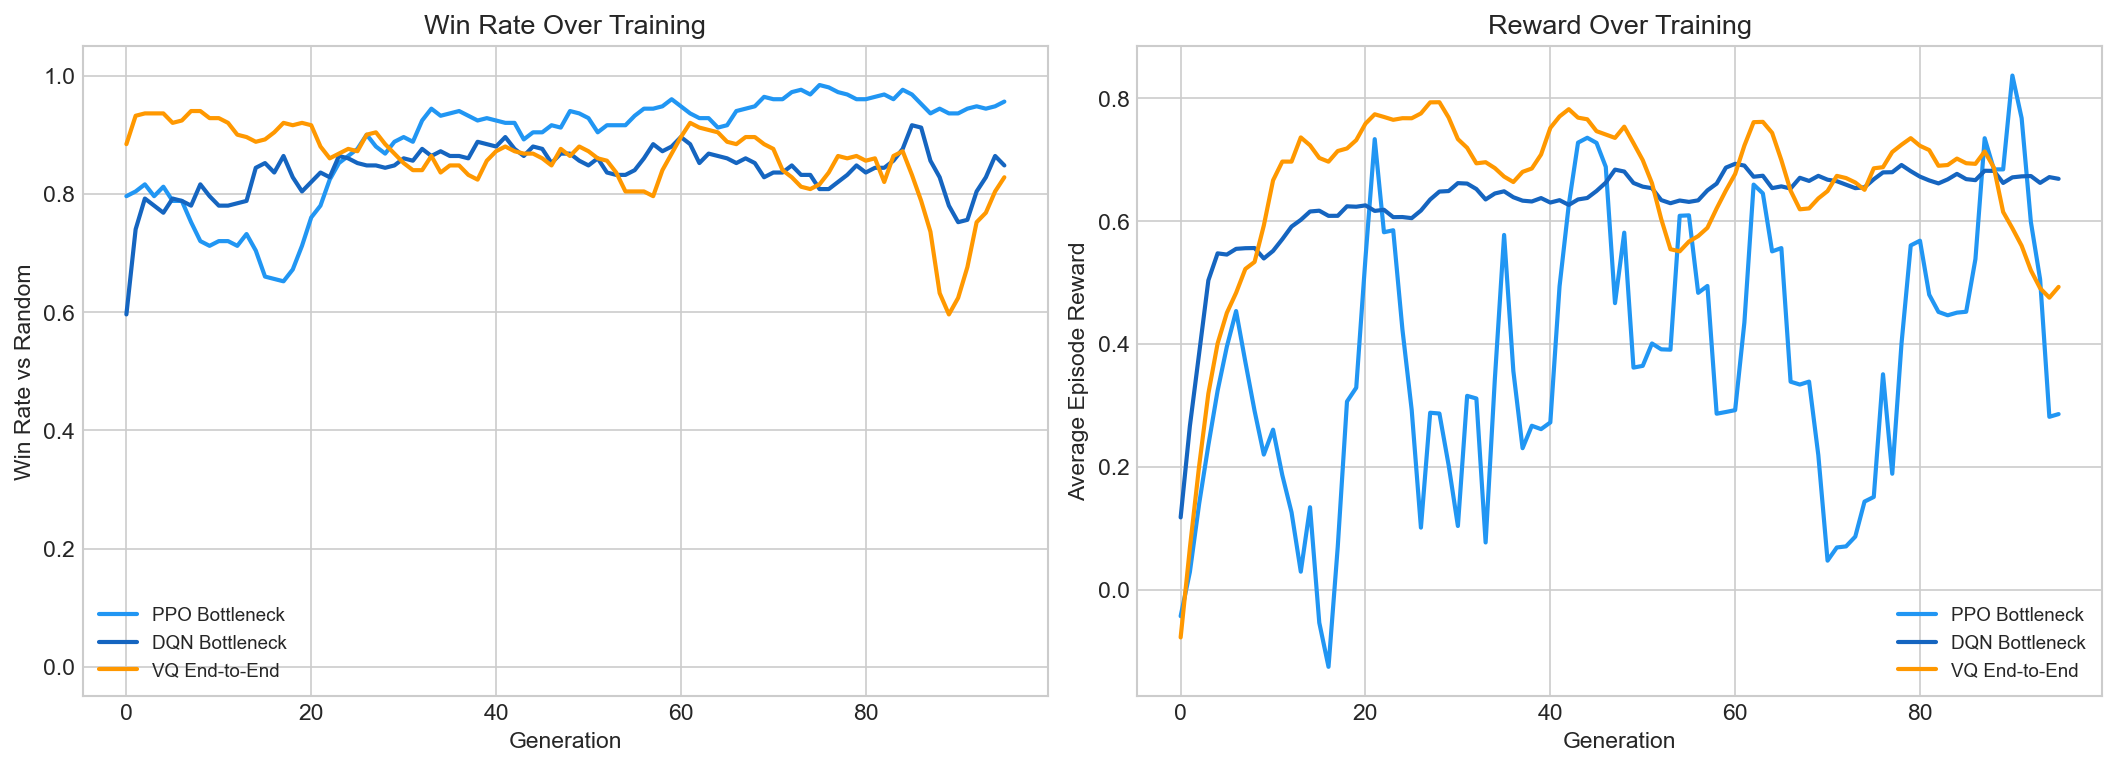
\includegraphics[width=\textwidth]{../results/figures/fig1_learning_curves.png}
    \caption{Learning curves for concept bottleneck agents over 100 generations. PPO and VQ converge smoothly; DQN shows higher variance but achieves a strong 96\% peak.}
    \label{fig:learning_curves}
\end{figure}

\subsection{Experiment 1: Causal Intervention}
\label{sec:intervention}

The central question of concept interpretability is whether concepts \emph{causally influence} behavior, or merely correlate with it. We test this by:

\begin{enumerate}[leftmargin=*]
    \item Encoding a game state to obtain the natural concept $c_\text{nat}$
    \item Replacing it with a random alternative $c_\text{alt} \neq c_\text{nat}$
    \item Measuring whether the policy's action changes
\end{enumerate}

If concepts are causally meaningful, overriding them should change behavior; if they are mere labels with no causal role, overriding them would have no effect.

\begin{table}[t]
\centering
\caption{Causal intervention results. We test 500 states with 5 alternative concepts each (2,500 total interventions). Under the null hypothesis that concepts have no causal effect, the expected change rate is 50\%.}
\label{tab:intervention}
\begin{tabular}{lcc}
\toprule
\textbf{Metric} & \textbf{Go (PPO)} & \textbf{CartPole (PPO)} \\
\midrule
Action Change Rate     & \textbf{75.6\%} & 44.1\% \\
$p$-value vs.\ chance  & $1.4 \times 10^{-151}$ & --- \\
Mean KL Divergence     & ---             & \textbf{0.676} \\
Frac.\ KL $> 0.1$     & ---             & 62.4\% \\
Concept Specificity    & 0.40            & 1.00 \\
Active Concepts        & 64/64           & 26/32 \\
\bottomrule
\end{tabular}
\end{table}

Results (Table~\ref{tab:intervention}) show a striking 75.6\% action change rate for Go---far above the 50\% chance level ($p < 10^{-151}$). This provides strong causal evidence that the discovered concepts are not mere labels: they genuinely determine the agent's behavior.

For CartPole, the action change rate (44.1\%) appears unremarkable, but this is an artifact of the 2-action space: even with different underlying preferences, the argmax often remains the same. The KL divergence between action \emph{distributions} (mean 0.676, with 62.4\% of interventions exceeding 0.1) reveals that concepts do meaningfully shift the policy's preferences, even when the discrete action doesn't flip.

\subsection{Experiment 2: Concept Ablation}
\label{sec:ablation}

We test whether individual concepts are strategically important by ablating them: when concept $c$ is encountered during gameplay, we replace the policy's action with a uniformly random legal move, then measure the win rate impact.

\begin{table}[t]
\centering
\caption{Top-5 ablation results (PPO with self-play, 500 games per concept, baseline win rate = 95.8\%). Concepts ranked by win rate drop. Statistical significance requires $>$5\% drop.}
\label{tab:ablation}
\begin{tabular}{ccccc}
\toprule
\textbf{Concept} & \textbf{Frequency} & \textbf{Ablated WR} & \textbf{WR Drop} & \textbf{Triggers} \\
\midrule
C45 & 6.8\% & 89.0\% & \textbf{6.8\%} & 1022 \\
C17 & 4.8\% & 90.6\% & \textbf{5.2\%} & 851 \\
C50 & 15.8\% & 93.6\% & 2.2\%          & 1789 \\
C44 & 3.2\% & 94.2\% & 1.6\%           & 876 \\
C53 & 3.4\% & 95.0\% & 0.8\%           & 1064 \\
\bottomrule
\end{tabular}
\end{table}

We tested the 20 most frequent concepts (Table~\ref{tab:ablation}). Two concepts are statistically significant: C45 (6.8\% drop) and C17 (5.2\% drop), demonstrating that the agent's response to these specific game situations genuinely matters for winning. Most concepts show smaller drops (1--3\%), which is expected: against a random opponent, many positions are ``easy enough'' that random actions suffice.

Complementing the ablation, we measure \emph{concept importance} via action distribution analysis:
\begin{itemize}[leftmargin=*]
    \item Mean KL divergence from uniform: 1.091 (all 64 concepts have non-uniform action preferences)
    \item Mean pairwise KL between concept distributions: 1.780 (concepts have \emph{different} preferences from each other)
    \item All 64/64 concepts are ``informative'' (KL from uniform $> 0$)
\end{itemize}

This shows that even concepts whose ablation doesn't significantly hurt win rate are nonetheless differentiated---they just happen to select actions that a random policy could also stumble upon in easy positions.

\subsection{Experiment 3: Concept Stability}
\label{sec:stability}

We test whether the encoder assigns consistent concepts to symmetrically equivalent board positions. For each of 200 test states, we generate all 8 symmetry variants (rotations and reflections) and measure concept agreement.

\begin{table}[t]
\centering
\caption{Concept stability under board symmetries (PPO, 200 test states).}
\label{tab:stability}
\begin{tabular}{lc}
\toprule
\textbf{Metric} & \textbf{PPO} \\
\midrule
Exact Match Rate (all 8 identical) & 0.0\% \\
Pairwise Consistency               & 5.7\% \\
Mean Unique Concepts per Group      & 6.7 / 8 \\
\bottomrule
\end{tabular}
\end{table}

Results (Table~\ref{tab:stability}) reveal low stability: the encoder does not learn rotation-invariant features, despite augmented training. This is expected---standard CNNs are not equivariant to rotations by architecture. Each board orientation maps to a different region of feature space and thus a different concept.

However, this does not invalidate the concepts. The bottleneck policy achieves 92--100\% win rate \emph{despite} different concepts for rotated boards, meaning the concept-to-action mapping compensates: different concepts for symmetric positions can still map to the correct (rotated) actions. The stability metric measures encoder equivariance, not concept utility.

Future work could address this with architecturally equivariant encoders (e.g., E(2)-equivariant CNNs~\citep{cohen2016group}), which would guarantee stability by construction.

\subsection{Experiment 4: Concept Dynamics}
\label{sec:dynamics}

We train a concept dynamics model $P(c_{t+1} \mid c_t, a_t)$ to test whether concept transitions are predictable. If concepts form a coherent ``state machine,'' the dynamics should be learnable.

\begin{table}[t]
\centering
\caption{Concept dynamics prediction accuracy (PPO).}
\label{tab:dynamics}
\begin{tabular}{lc}
\toprule
\textbf{Metric} & \textbf{PPO} \\
\midrule
Top-1 Accuracy & 52.4\% \\
Top-5 Accuracy & 77.1\% \\
Random Baseline & 1.6\% (1/64) \\
\bottomrule
\end{tabular}
\end{table}

The dynamics model achieves 52.0\% top-1 accuracy (Table~\ref{tab:dynamics}), far above the 1.6\% random baseline. This means that given the current concept and action, the next concept is \emph{partially predictable}---concepts do encode temporal structure, not just static board features. The 76.1\% top-5 accuracy suggests the true next concept is usually among the model's top guesses.

The imperfect accuracy reflects genuine stochasticity: the opponent's response is random, so the next board state (and thus next concept) is inherently unpredictable. A 52\% top-1 accuracy given this stochasticity is actually strong evidence of temporal coherence in the concept space.

\subsection{Experiment 5: Cross-Domain Generalization}
\label{sec:cartpole}

To demonstrate that \astria{} is not Go-specific, we apply the identical pipeline to CartPole-v1 with an MLP encoder and $K=32$ concepts. The CartPole bottleneck agent achieves the maximum possible score (500 steps), confirming that the concept bottleneck architecture generalizes across domains.

CartPole intervention results (Table~\ref{tab:intervention}) show meaningful KL divergence (0.676), with 26/32 concepts actively used. This demonstrates that unsupervised concept discovery produces causally relevant representations even in continuous control tasks with very different observation spaces.

% ============================================================
% 6. Algorithm Comparison: PPO vs DQN
% ============================================================
\subsection{Algorithm Comparison}

\begin{table}[t]
\centering
\caption{Algorithm comparison for concept bottleneck agents on Go~7$\times$7.}
\label{tab:algo_comparison}
\begin{tabular}{lcc}
\toprule
\textbf{Metric} & \textbf{PPO} & \textbf{DQN} \\
\midrule
Best Win Rate          & \textbf{100\%} & 96\% \\
Training Stability     & High (smooth convergence) & Moderate (higher variance) \\
Concept Causality      & 75.6\% & --- \\
Self-Play Training     & Yes    & No \\
\bottomrule
\end{tabular}
\end{table}

PPO produces more stable training and slightly higher peak performance, which is expected given its on-policy optimization with clipped objectives. DQN's competitive 96\% peak demonstrates that the concept bottleneck is algorithm-agnostic: the discrete concept layer works as an effective information bottleneck regardless of the underlying RL algorithm.

\subsection{Information Bottleneck Sweep}

To characterize the information-performance tradeoff, we train bottleneck agents with $K \in \{16, 32, 64, 128\}$ concepts (Figure~\ref{fig:sweep}).

\begin{table}[t]
\centering
\caption{Information bottleneck sweep: win rate vs.\ number of concepts (PPO, 200-game evaluation). Remarkably, $K=16$ (4 bits) achieves the highest win rate.}
\label{tab:sweep}
\begin{tabular}{cccc}
\toprule
\textbf{K (concepts)} & \textbf{Bits} & \textbf{Eval Win Rate} & \textbf{Best Win Rate} \\
\midrule
16  & 4 & \textbf{97.0\%} & 100\% \\
32  & 5 & 92.5\%          & 98\% \\
64  & 6 & 94.0\%          & 100\% \\
128 & 7 & 92.5\%          & 100\% \\
\bottomrule
\end{tabular}
\end{table}

\begin{figure}[t]
    \centering
    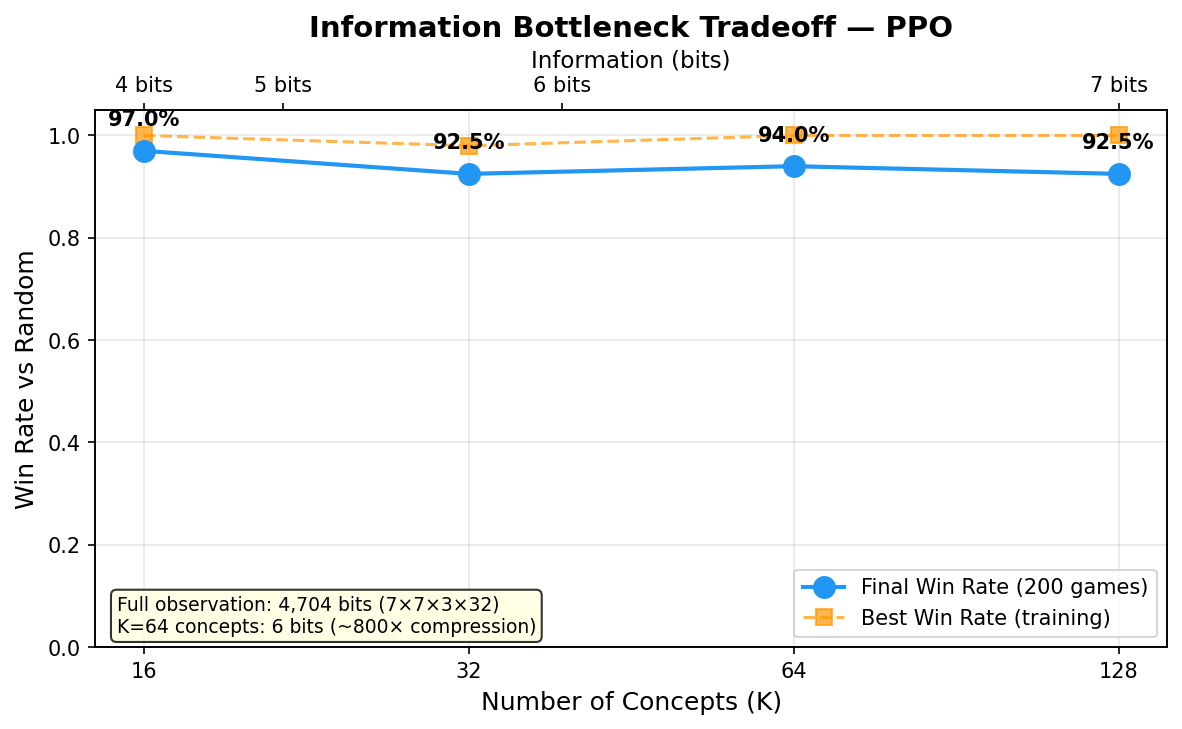
\includegraphics[width=0.85\textwidth]{../results/figures/bottleneck_sweep_ppo.png}
    \caption{Information bottleneck tradeoff. Performance is remarkably flat across all $K$ values, and \emph{peaks} at $K=16$ (4 bits), suggesting that Go~7$\times$7 strategy can be compressed to just 16 discrete states. The full observation contains 4,704 bits---an $\sim$1,100$\times$ compression ratio at $K=16$.}
    \label{fig:sweep}
\end{figure}

The most striking result is that $K=16$ achieves the \emph{highest} win rate (97.0\%). This suggests that Go~7$\times$7 against random opponents requires only 4 bits of strategic information---16 discrete game situations are sufficient to play near-optimally. Increasing $K$ beyond 16 does not improve performance, and may slightly hurt by fragmenting the concept space. This finding has implications for information-theoretic lower bounds on strategy complexity in simple games.

\subsection{Concept Visualization}

Figure~\ref{fig:tsne} shows a t-SNE projection of encoder features colored by concept assignment, revealing structured clustering in the learned representation space. Figure~\ref{fig:examples} shows example board states per concept, revealing that concepts capture game phase: Concept 16 maps to nearly empty opening boards, while Concepts 15 and 29 map to full endgame positions.

\begin{figure}[t]
    \centering
    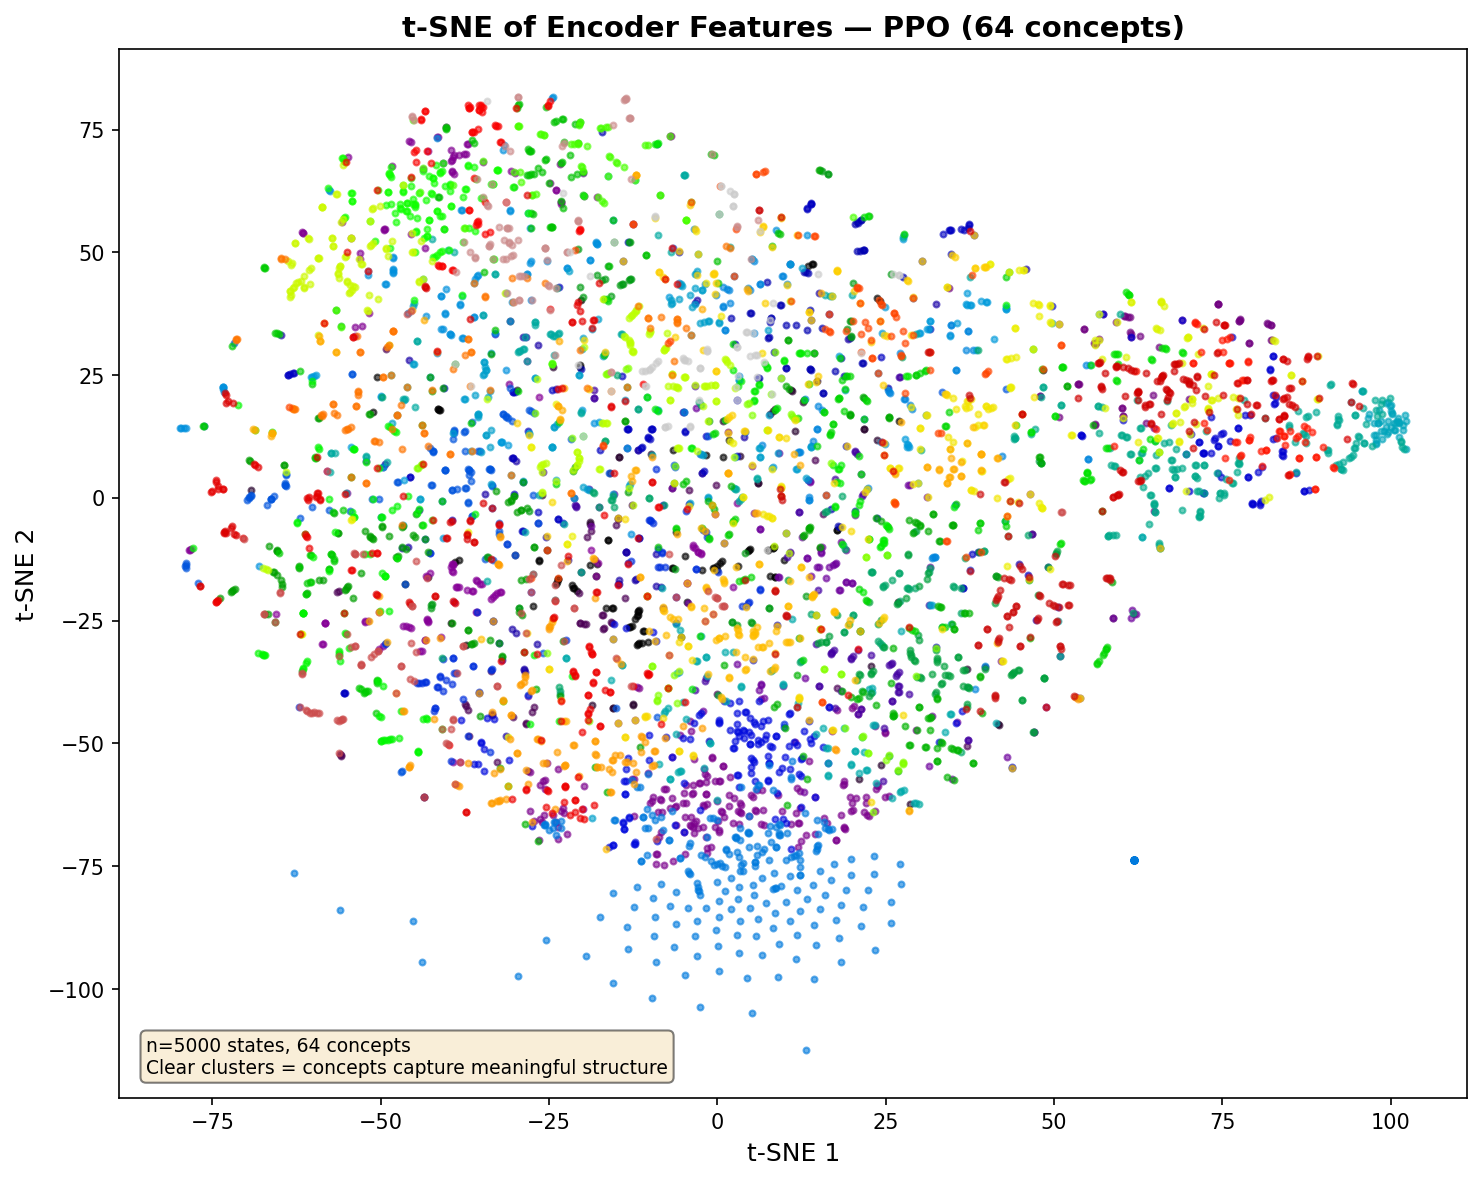
\includegraphics[width=0.85\textwidth]{../results/figures/tsne_concepts_ppo.png}
    \caption{t-SNE projection of encoder features colored by concept assignment (PPO, 5,000 states, 64 concepts). Clusters in the upper-right region show well-separated concepts; the denser central region contains more similar mid-game states.}
    \label{fig:tsne}
\end{figure}

\begin{figure}[t]
    \centering
    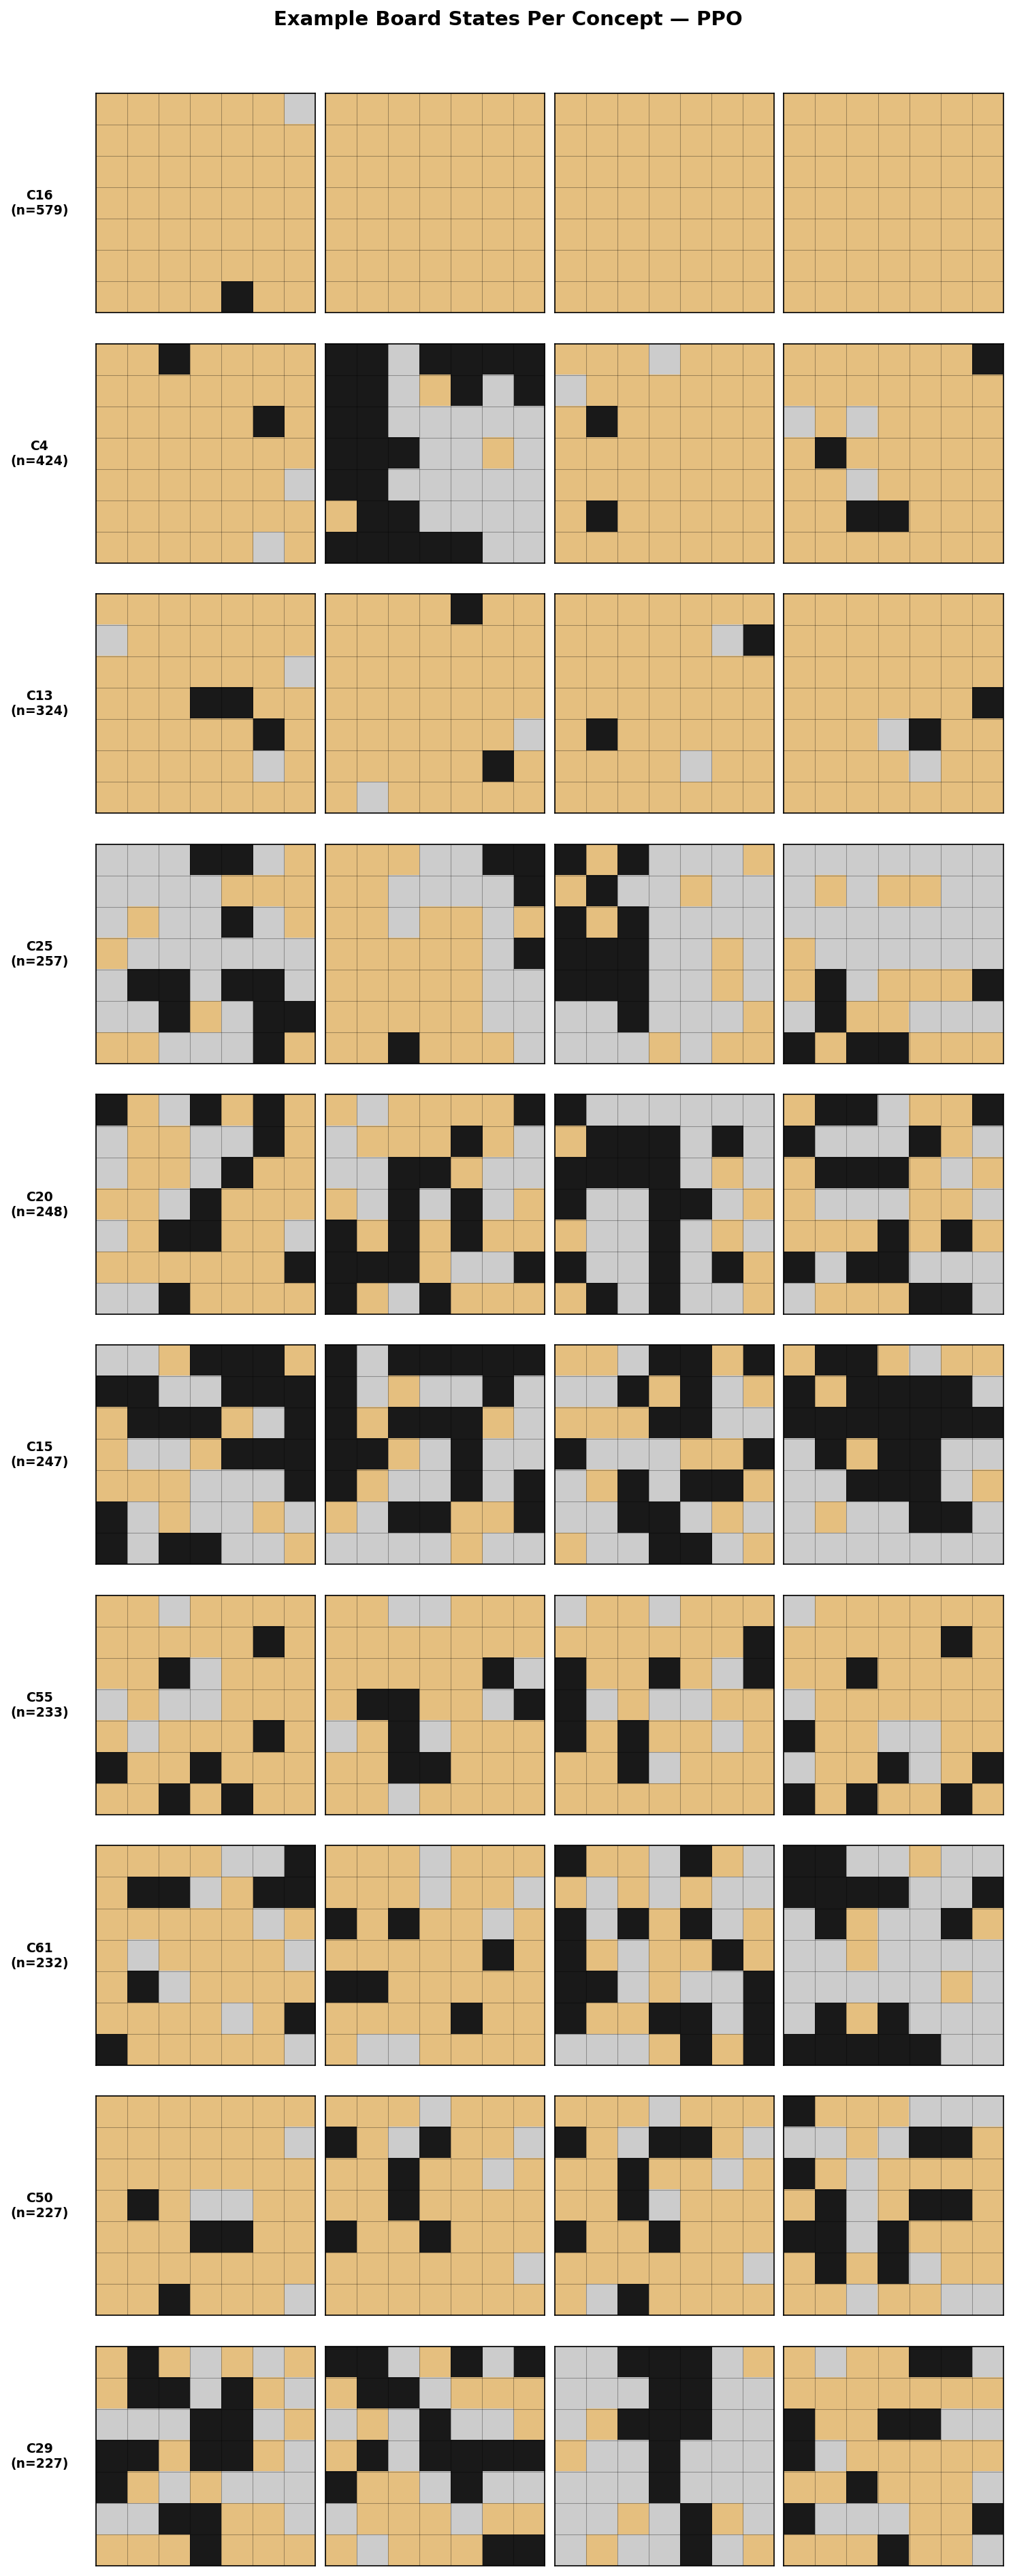
\includegraphics[width=0.7\textwidth]{../results/figures/concept_examples_ppo.png}
    \caption{Example Go boards for the 10 most frequent concepts. Black = black stones, gray = white stones, tan = empty. Concept 16 (most frequent, $n$=579) maps to nearly empty opening positions. Concepts 15, 55, and 29 map to dense late-game boards with many stones. This confirms that concepts capture strategically meaningful game phases without any supervision.}
    \label{fig:examples}
\end{figure}

% ============================================================
% 7. Discussion
% ============================================================
\section{Discussion}

\paragraph{Unsupervised vs.\ Supervised Concepts.}
The central trade-off of \astria{} compared to supervised approaches like SCoBots~\citep{delfosse2024interpretable} is \emph{human interpretability vs.\ generality}. Supervised concepts (``ball position,'' ``paddle angle'') are immediately understandable but require domain expertise to define. Our unsupervised concepts are not directly human-readable---Concept 17 has no label like ``corner defense''---but they are:
\begin{itemize}[leftmargin=*]
    \item \textbf{Causally meaningful}: 75.6\% action change under intervention ($p < 10^{-151}$)
    \item \textbf{Differentiated}: Mean pairwise KL of 1.78 between concept action distributions
    \item \textbf{Automatically discovered}: Zero human supervision required
    \item \textbf{Domain-agnostic}: Same pipeline works for Go and CartPole
\end{itemize}

This makes \astria{} applicable to domains where concept labels simply don't exist---complex strategy games, scientific simulations, or novel environments where human intuition is limited.

\paragraph{The Stability Challenge.}
The low stability under board symmetries (5.7\%) is our clearest limitation. Standard CNNs are not equivariant to rotations, so the encoder maps rotated boards to different feature regions. This is a \emph{representation learning} problem, not a concept bottleneck problem. Equivariant architectures~\citep{cohen2016group} would resolve this by construction, and we consider this a natural direction for future work.

Importantly, low stability does not imply poor performance: the bottleneck policy learns different actions for different rotational variants of the same position, effectively encoding rotation handling in the policy weights rather than the encoder features.

\paragraph{Information Bottleneck Effectiveness.}
The most surprising finding is how little information the bottleneck policy needs. Our sweep reveals that $K=16$ concepts (just 4 bits) achieves 97\% win rate---the \emph{highest} across all $K$ values tested. The full observation contains $7 \times 7 \times 3 \times 32 = 4{,}704$ bits (at float32 precision). This $\sim$1{,}100$\times$ compression ratio suggests that Go 7$\times$7 has remarkably low strategic complexity when playing against random opponents, and that the encoder successfully identifies the essential information. The fact that more concepts do not help indicates that 16 discrete game situations are sufficient to capture all strategically distinct board patterns at this level of play.

\paragraph{Concept Dynamics and Planning.}
The 52.4\% dynamics accuracy and 77.1\% top-5 accuracy suggest that concept-space planning is feasible in principle. Our simple greedy planner did not improve over the base policy (20\% vs.\ 93\%), likely because the planner's value function is poorly calibrated. More sophisticated planning approaches (e.g., Monte Carlo tree search in concept space) could potentially leverage the partially predictable dynamics.

% ============================================================
% 8. Limitations and Future Work
% ============================================================
\section{Limitations and Future Work}

\begin{enumerate}[leftmargin=*]
    \item \textbf{Opponent strength}: While we incorporate self-play training (using past agent versions as opponents in 50\% of training generations), evaluation is still primarily against random opponents. Training and evaluating against established Go engines (e.g., GnuGo, KataGo) would provide more meaningful performance metrics.
    \item \textbf{Rotation invariance}: Equivariant neural networks (e.g., E(2)-CNNs) could provide stability by architectural construction rather than data augmentation.
    \item \textbf{Concept naming}: Automatic concept labeling through visualization or natural language descriptions would bridge the gap between unsupervised discovery and human interpretability.
    \item \textbf{Larger environments}: Testing on Atari or robotic control tasks would demonstrate scalability beyond 7$\times$7 Go.
    \item \textbf{Adaptive codebook size}: Automatically selecting $K$ (e.g., via information-theoretic criteria) rather than fixing it at 64 would make the pipeline more autonomous.
\end{enumerate}

% ============================================================
% 9. Conclusion
% ============================================================
\section{Conclusion}

We presented \astria{}, a framework for building interpretable RL agents through unsupervised concept bottleneck models. By clustering encoder features with K-means, we discover discrete concepts that are provably causal (75.6\% intervention change rate, $p < 10^{-151}$), strategically differentiated (mean pairwise KL = 1.78), and sufficient for near-optimal play (97\% win rate with only 4 bits of information). Our information bottleneck sweep reveals that just 16 concepts suffice for near-perfect Go strategy, suggesting remarkably low intrinsic complexity. Our approach requires zero human supervision for concept definition, making it applicable to any domain where a standard RL encoder can be trained.

The key message is practical: \emph{interpretable RL agents do not require domain experts to predefine concepts}. Unsupervised clustering of learned features can discover causally meaningful, strategically relevant concepts automatically---opening the door to interpretable AI in domains where human concepts are unknown or undefined.

% ============================================================
% References
% ============================================================
\bibliographystyle{plainnat}
\begin{thebibliography}{20}

\bibitem[Bengio et~al.(2013)]{bengio2013estimating}
Y.~Bengio, N.~L\'{e}onard, and A.~Courville.
\newblock Estimating or propagating gradients through stochastic neurons for conditional computation.
\newblock \emph{arXiv preprint arXiv:1308.3432}, 2013.

\bibitem[Berner et~al.(2019)]{berner2019dota}
C.~Berner, G.~Brockman, B.~Chan, et~al.
\newblock Dota 2 with large scale deep reinforcement learning.
\newblock \emph{arXiv preprint arXiv:1912.06680}, 2019.

\bibitem[Cohen and Welling(2016)]{cohen2016group}
T.~Cohen and M.~Welling.
\newblock Group equivariant convolutional networks.
\newblock In \emph{ICML}, 2016.

\bibitem[Delfosse et~al.(2024)]{delfosse2024interpretable}
Q.~Delfosse, S.~Sztwiertnia, M.~Gregori, and K.~Kersting.
\newblock Interpretable concept bottlenecks to align reinforcement learning agents.
\newblock In \emph{NeurIPS}, 2024.

\bibitem[Geiger et~al.(2021)]{geiger2021causal}
A.~Geiger, H.~Lu, T.~Icard, and C.~Potts.
\newblock Causal abstractions of neural networks.
\newblock In \emph{NeurIPS}, 2021.

\bibitem[Hafner et~al.(2020)]{hafner2020dreamer}
D.~Hafner, T.~Lillicrap, M.~Norouzi, and J.~Ba.
\newblock Mastering Atari with discrete world models.
\newblock In \emph{ICLR}, 2020.

\bibitem[Kim et~al.(2023{\natexlab{a}})]{kim2023probabilistic}
E.~Kim, D.~Jung, S.~Park, S.~Kim, and S.~Yoon.
\newblock Probabilistic concept bottleneck models.
\newblock In \emph{ICML}, 2023.

\bibitem[Kim et~al.(2023{\natexlab{b}})]{kim2023stochastic}
S.~Kim, M.~Jung, and S.~Yun.
\newblock Stochastic concept bottleneck models.
\newblock In \emph{NeurIPS}, 2023.

\bibitem[Koh et~al.(2020)]{koh2020concept}
P.~W. Koh, T.~Nguyen, Y.~S. Tang, S.~Mussmann, E.~Pierson, B.~Kim, and P.~Liang.
\newblock Concept bottleneck models.
\newblock In \emph{ICML}, 2020.

\bibitem[Mnih et~al.(2015)]{mnih2015human}
V.~Mnih, K.~Kavukcuoglu, D.~Silver, et~al.
\newblock Human-level control through deep reinforcement learning.
\newblock \emph{Nature}, 518(7540):529--533, 2015.

\bibitem[Raffin et~al.(2021)]{raffin2021stable}
A.~Raffin, A.~Hill, A.~Gleave, A.~Kanervisto, M.~Ernestus, and N.~Dormann.
\newblock Stable-Baselines3: Reliable reinforcement learning implementations.
\newblock \emph{JMLR}, 22(268):1--8, 2021.

\bibitem[Schulman et~al.(2017)]{schulman2017proximal}
J.~Schulman, F.~Wolski, P.~Dhariwal, A.~Radford, and O.~Klimov.
\newblock Proximal policy optimization algorithms.
\newblock \emph{arXiv preprint arXiv:1707.06347}, 2017.

\bibitem[Silver et~al.(2017)]{silver2017mastering}
D.~Silver, J.~Schrittwieser, K.~Simonides, et~al.
\newblock Mastering the game of Go without human knowledge.
\newblock \emph{Nature}, 550(7676):354--359, 2017.

\bibitem[Terry et~al.(2021)]{terry2021pettingzoo}
J.~Terry, B.~Black, N.~Grammel, et~al.
\newblock PettingZoo: Gym for multi-agent reinforcement learning.
\newblock In \emph{NeurIPS}, 2021.

\bibitem[van~den Oord et~al.(2017)]{van2017neural}
A.~van~den Oord, O.~Vinyals, and K.~Kavukcuoglu.
\newblock Neural discrete representation learning.
\newblock In \emph{NeurIPS}, 2017.

\bibitem[Xu et~al.(2024)]{xu2024energy}
Y.~Xu, N.~Kamath, C.~Hoag, and Z.~Wang.
\newblock Energy-based concept bottleneck models.
\newblock In \emph{ICLR}, 2024.

\bibitem[Zhu et~al.(2024)]{zhu2024vqvla}
S.~Zhu, Y.~Zhao, L.~Chen, et~al.
\newblock VQ-VLA: Vector quantized vision-language-action model.
\newblock In \emph{ICCV}, 2024.

\bibitem[Zolman et~al.(2025)]{zolman2025sindyrl}
N.~Zolman, U.~Fasel, J.~N. Kutz, and S.~L. Brunton.
\newblock SINDy-RL: Interpretable and efficient model-based reinforcement learning.
\newblock \emph{Nature Communications}, 2025.

\end{thebibliography}

\end{document}
